\documentclass[english,hidelinks,pdftex, 11 pt, class=article,crop=false]{standalone}
\usepackage[T1]{fontenc}
\usepackage[utf8]{luainputenc}
\usepackage{lmodern} % load a font with all the characters
\usepackage{geometry}
\geometry{verbose,a4paper, inner=0cm, outer=0 cm, bmargin=2cm, tmargin=1cm}
%\textwidth=12cm
\setlength{\parindent}{0bp}
\usepackage{import}
\usepackage[subpreambles=false]{standalone}
\usepackage{amsmath}
\usepackage{amssymb}
\usepackage{esint}
\usepackage{babel}
\usepackage{tabu}
\usepackage[dvipsnames, table]{xcolor}
\usepackage{cancel}
\makeatother
\makeatletter
\usepackage{datetime2}
\usepackage{titlesec}
\usepackage[many]{tcolorbox}

% Eheter
\newcommand{\enh}[1]{\,\textrm{#1}}
%referances
\newcommand{\net}[2]{{\color{blue}\href{#1}{#2}}}

%Spaces
\newcommand{\vsk}{\\[12pt]}
\newcommand{\vs}{\vspace{-12pt}}

% Tabell for opplegg

\newcommand{\ovlist}[1]{
\vspace{-16pt}
\begin{itemize}
	#1
\end{itemize}
}

% Chapters and sections
\titleformat{\section}[block]{\bfseries}{\hspace{3cm}\thesection}{5pt}{}
\titleformat{\subsection}[block]{\bfseries}{\hspace{3cm}\thesection}{5pt}{}
\newcommand{\sectionbreak}{\clearpage} % New page on each section
 

\newlength{\mywidth}
\setlength{\mywidth}{14cm}

\newcommand{\cont}[1]{
\begin{tcolorbox}[center, boxrule=0.0 mm, width=\mywidth,arc=0mm,enhanced jigsaw,,colback=white,breakable]
#1	
\end{tcolorbox}
}

\newcommand{\info}[5]{
\begin{tcolorbox}[center, boxrule=0.1 mm, width=\mywidth,arc=0mm,enhanced jigsaw,breakable,colback=yellow!5]	
	
	\footnotesize
	\textbf{Øvingsområde}\\[5pt] #1 
	
	\textbf{Utstyr}\\ #2  \\
	
	\begin{tabular}{@{} p{4cm} p{4cm} l} 
		\textbf{Tid} & \textbf{Elevinndeling} & \textbf{Læringsarena} \\
		#3  & #4 & #5
	\end{tabular} 
\end{tcolorbox}	
}

\newcommand{\gjen}[1]{\begin{tcolorbox}[center,boxrule=0.1 mm, width=\mywidth,arc=0mm,colback=blue!3] {\large \textbf{Gjennomføring} \vspace{5 pt}}\newline #1  \end{tcolorbox}\vspace{-5pt}}
\newcommand{\eks}[1]{\begin{tcolorbox}[center,boxrule=0.1 mm, width=\mywidth,arc=0mm,colback=green!3] {\large \textbf{Eksempel} \vspace{5 pt}}\newline #1  \end{tcolorbox}\vspace{-5pt}}

\newcounter{opl}
%\numberwithin{opl}{article}


\newcommand{\opl}[1]{
\newpage
{\refstepcounter{opl} %\phantomsection 
\large \textbf{\theopl \;#1} \vsk}
}

% Headlines
\newcommand{\fork}{\textbf{Forkunnskapar}\\}
\newcommand{\forb}{\textbf{Forberedelsar}\\}
\newcommand{\opgvr}{\textbf{Oppgaver}}



%colors
\newcommand{\colr}[1]{{\color{red} #1}}
\newcommand{\colb}[1]{{\color{blue} #1}}
\newcommand{\colo}[1]{{\color{orange} #1}}
\newcommand{\colc}[1]{{\color{cyan} #1}}
\definecolor{projectgreen}{cmyk}{100,0,100,0}
\newcommand{\colg}[1]{{\color{projectgreen} #1}}

% Lister med bokstavar
\usepackage[inline]{enumitem}
% Opg
\newcommand{\abc}[1]{
	\begin{enumerate}[label=\alph*),leftmargin=18pt]
		#1
	\end{enumerate}
}

\usepackage[]{hyperref}


\renewcommand{\info}[2]{\begin{tcolorbox}[boxrule=0.3 mm,arc=0mm,enhanced jigsaw,breakable,colback=black!1] {\large \textbf{#1} \vspace{5 pt}\\} #2 \end{tcolorbox}\vspace{-5pt} }

\begin{document}

\begin{center}
	\huge \textbf{Trekantar}
\end{center}
\info{Rettvinka trekant}{
 Éin av vinklane er $ 90^\circ $.
\begin{wrapfigure}{r}{0.4\textwidth}
	\vspace{-40pt}
	\includegraphics[]{rettvinklet}
\end{wrapfigure}

\vspace{50pt}
}
\info{Likesida trekant}{
	Alle sidene er like lange. \vsk
	
	Alle vinklane er $ 60^\circ $.
	\begin{wrapfigure}{r}{0.35\textwidth}
		\vspace{-70pt}
		\includegraphics[]{likesidet}
	\end{wrapfigure}
	
	\vspace{40pt}
}
\info{Likebeint trekant}{
	To sider er like lange. \vsk
	
	To vinklar er like store.
	\begin{wrapfigure}{r}{0.35\textwidth}
		\vspace{-70pt}
		\includegraphics[]{likebeint}
	\end{wrapfigure}
	
	\vspace{50pt}
}
\newpage
\begin{center}
	\huge \textbf{Firkantar}
\end{center}
\info{Kvadrat}{
	Alle sidene er like lange. \vsk
	
	Alle vinklane er $ 90^\circ $.
	\begin{wrapfigure}{r}{0.35\textwidth}
		\vspace{-70pt}
		\includegraphics[]{kvadrat}
	\end{wrapfigure}
\vspace{20pt}
}
\info{Rektangel}{
	To og to sider er like lange. \vsk
	
	Alle vinklane er $ 90^\circ $. 
	\begin{wrapfigure}{r}{0.35\textwidth}
		\vspace{-65pt}
		\includegraphics[]{rektangel}
	\end{wrapfigure}
}
\info{Rombe}{
	Alle sidene er like lange. \vsk
	
	To og to vinklar er like store. 
	\begin{wrapfigure}{r}{0.4\textwidth}
		\vspace{-70pt}
		\includegraphics[]{rombe}
	\end{wrapfigure}
\vspace{10pt}
}
\info{Trapes}{
	To av sidene er parallelle. 
	\begin{wrapfigure}{r}{0.45\textwidth}
		\vspace{-45pt}
		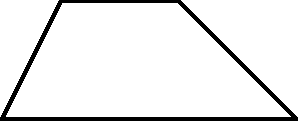
\includegraphics[]{trapes}
	\end{wrapfigure}
\vspace{20pt}
}
\info{Parallellogram}{
	To og to sider er like lange. \vsk
	
	To og to vinklar er like store. \vsk
	
	To og to sider er parallelle.
	\begin{wrapfigure}{r}{0.52\textwidth}
		\vspace{-95pt}
		\includegraphics[]{parallellogram}
	\end{wrapfigure}
\vspace{10pt}
}
\end{document}

